\chapter{Судалгааны үр дүн}
\label{ch:results}

\section{Хэрэгжилтийн үр дүнгийн тойм}

Энэхүү судалгааны хүрээнд AI Notebook системийн харагдах хэсэг (frontend), сервер талын хэсэг (backend), өгөгдлийн сан, хиймэл оюуны интеграц гэсэн үндсэн бүрэлдэхүүнүүд бүрэн хэрэгжиж, хоорондын уялдаа ажиллах түвшинд хүрсэн. Үр дүнг системийн түвшинд авч үзвэл:

\begin{enumerate}
    \item Хэрэглэгчийн баталгаажуулалтын урсгал амжилттай,
    \item Тэмдэглэлийн амьдралын мөчлөг (note lifecycle: үүсгэх-засах-устгах) тогтвортой,
    \item Календарь болон сэтгэл хөдлөлийн төлөвөөр (mood) тэмдэглэл харах боломж хэрэгжсэн,
    \item Хиймэл оюун ухаанаар стикер үүсгэх (AI sticker generation) төгсгөлийн цэг амжилттай интеграцчлагдсан,
    \item JWT завсрын модуль (middleware)-аар хамгаалагдсан API зохих ёсоор ажилласан.
\end{enumerate}

\section{Өгөгдлийн урсгалын зурагт суурилсан баталгаажуулалт (dataflow)}

Арга зүйн бүлэгт тодорхойлсон \fref{fig:dfd_context}, \fref{fig:dfd_level1}, \fref{fig:dfd_auth_detail}, \fref{fig:dfd_notes_detail}, \fref{fig:dfd_sticker_detail} диаграммууд дээрх урсгал бүрийг бодит кодын зан төлөвтэй харьцуулан шалгав.

\begin{table}[H]
\centering
\caption{Өгөгдлийн урсгалын түвшний баталгаажуулалтын нэгтгэл}
\label{tab:dataflow_validation}
\begin{tabular}{>{\raggedright\arraybackslash}p{3.8cm}>{\raggedright\arraybackslash}p{6.5cm}>{\raggedright\arraybackslash}p{2.8cm}}
\toprule
\textbf{Урсгал} & \textbf{Баталгаажсан шалгалт} & \textbf{Дүн} \\
\midrule
Баталгаажуулалтын урсгал (Auth flow) & /api/auth/login, /api/auth/signup урсгалд токен болон хэрэглэгчийн мэдээлэл буцаж, хамгаалалттай санах ойд (Secure Storage) хадгалагдсан & Амжилттай \\
Тэмдэглэлийн урсгал (Notes flow) & /api/notes төрлийн CRUD хүсэлт бүр завсрын модуль (middleware)-ээр дамжин зөвхөн тухайн хэрэглэгчийн өгөгдөлд үйлчилсэн & Амжилттай \\
Наалт зургийн урсгал (Sticker flow) & /api/notes/generate-sticker урсгал заавар текст (prompt) авч OpenAI руу дамжуулан наалт зургийн URL буцаасан & Амжилттай \\
Алдааны урсгал (Error flow) & API түлхүүр (key), хязгаарлалт (quota), сүлжээний (network) алдааг харагдах хэсэгт (frontend) тайлбартай мессеж (snackbar) болгон харуулсан & Амжилттай \\
\bottomrule
\end{tabular}
\end{table}

\section{Дарааллын диаграммын түвшний баталгаажуулалт (sequence)}

\fref{fig:seq_login}, \fref{fig:seq_note_create}, \fref{fig:seq_sticker} гэсэн дарааллын (sequence) диаграммуудаар харуулсан хугацааны дарааллыг туршилтаар дараах байдлаар баталгаажуулав.

\begin{enumerate}
    \item Нэвтрэх (login) үед хэрэглэгч шалгах, нууц үгийг баталгаажуулах, токен үүсгэх дараалал хэвийн ажилласан. Үүний дараа дотоод хадгалалт шинэчлэгдсэн.
    \item Тэмдэглэл үүсгэх (note create) үед токен баталгаажуулах, хэрэглэгчийн эрхийг тогтоох, өгөгдөл хадгалах, интерфейс шинэчлэх дараалал тасалдаагүй.
    \item Наалт зураг үүсгэх (sticker generate) үед заавар текст (prompt) шалгах, AI үйлчилгээ рүү дамжуулах, URL хариу буцаах дараалал тогтвортой ажилласан.
\end{enumerate}

\section{Харагдах хэсгийн (frontend) хөгжүүлэлтийн үр дүн}

Flutter дээрх харагдах хэсэгт (frontend) дараах үндсэн дэлгэцүүдийг бүтээсэн:

\begin{itemize}
    \item Нэвтрэх/бүртгэх (Login/Signup): Нэвтрэх болон бүртгэх урсгал.
    \item Хянах самбар (Dashboard): Өнөөдрийн тэмдэглэл, сэтгэл хөдлөлийн сонголт (mood picker), түргэн үйлдлүүд (quick actions).
    \item Календарь (Calendar): Огноогоор шүүлттэй тэмдэглэлийн харагдац.
    \item Наалт зураг (Sticker): Заавар текст (prompt) оруулж хиймэл оюун ухаанаар стикер үүсгэх (AI sticker generation).
    \item Мэдэгдлүүд (Notifications): Хэрэглэгчийн интерфейсийн (UI) түвшний мэдэгдлийн жагсаалт.
    \item Хувийн хэсэг (Profile): Хэрэглэгчийн мэдээлэл, системээс гарах (logout).
\end{itemize}

Навигаци (navigation) нь доод таб бүтэцтэй (bottom tab), \texttt{IndexedStack} ашигласнаар дэлгэц хооронд шилжих үед төлөв хадгалах нөхцөл бүрдсэн.

\section{Мэдэгдлийн (notification) модулийн хэрэгжилт}

Энэхүү системд мэдэгдлийн функцийг төхөөрөмжийн локал мэдэгдэл (local notification) болон апп доторх мэдэгдлийн төв (notification center) гэсэн хоёр түвшинд хэрэгжүүлсэн. Аппликейшн эхлэх үед мэдэгдлийн үйлчилгээ инициализаци хийгдэж, Android/iOS орчинд шаардлагатай зөвшөөрлүүдийг (permission) хүсэх механизмыг ажиллуулдаг. Android талд \texttt{sticker\_events\_channel} суваг үүсгэснээр сануулга, стикертэй холбоотой event-үүдийг тусгай сувгаар хүргэх боломж бүрдсэн.

Мэдэгдлийн урсгалын хувьд дараах үндсэн зан төлөв баталгаажсан.

\begin{itemize}
    \item Стикер үүссэний дараах мэдэгдэл: Наалт зураг (sticker) амжилттай үүсэхэд шууд мэдэгдэл үзүүлж, боломжтой үед зурагт суурилсан урьдчилан харах (big picture preview) хэлбэрээр харуулсан.
    \item Сануулга хуваарьлах (reminder scheduling): \texttt{reminderAt} талбарт суурилан тухайн тэмдэглэлд хамаарах мэдэгдлийг хугацаатайгаар хуваарьлаж, засвар/устгалын үед өмнөх хуваарийг цуцалж (cancel) дахин тохируулдаг.
    \item Мэдэгдлийн төв дэлгэц: Серверээс ирсэн тэмдэглэлийн өгөгдөл дундаас \texttt{reminderAt} эсвэл \texttt{stickerUrl} бүхий мөрүүдийг нэгтгэн мэдэгдлийн жагсаалт үүсгэж, уншсан/уншаагүй төлөв, устгах үйлдэл, таб дээрх тоон тэмдэг (badge)-тэй уялдуулсан.
\end{itemize}

Цагийн бүсийн (timezone) зөрүүгээс сэргийлэхийн тулд сануулгын хугацааг \texttt{TZDateTime.from(reminderAt.toUtc(), UTC)} хэлбэрээр хөрвүүлэн төлөвлөдөг шийдэл ашигласан нь төхөөрөмжийн орон нутгийн цагтай нийцтэй ажиллах нөхцөлийг сайжруулсан.

\section{Сервер талын хөгжүүлэлтийн үр дүн (backend)}

Node.js/Express дээрх сервер талын хэсэгт (backend) чиглүүлэлт (route) болон хянагч (controller)-ийг салгаж зохион байгуулсан нь системийн засварлах, өргөтгөх чадварыг (maintainability) сайжруулсан. Хэрэгжсэн боломжууд:

\begin{itemize}
    \item Баталгаажуулалтын API (Auth API): бүртгэл/нэвтрэлт (signup/login), bcrypt нууцлалын хэш (hash), JWT үүсгэлт.
    \item Тэмдэглэлийн API (Note API): үүсгэх, унших, шинэчлэх, устгах (create/read/update/delete).
    \item Наалт зургийн API (Sticker API): OpenAI-аар зураг үүсгэж URL буцаах.
    \item Эрхийн хяналт (Authorization): Bearer токен шалгах завсрын модуль (middleware).
\end{itemize}

MongoDB талд \texttt{User}, \texttt{Note} загваруудын талбарууд системийн бодит хэрэгцээг хангаж, нэмэлт атрибут өргөтгөх суурьтай болсон.

\section{Интеграцийн туршилтын үр дүн}

Функционал тестийн үр дүнг \tref{tab:test_result_summary} хүснэгтэд нэгтгэн харуулав.

\begin{table}[H]
\centering
\caption{Интеграцийн туршилтын үр дүнгийн нэгтгэл}
\label{tab:test_result_summary}
\begin{tabular}{>{\raggedright\arraybackslash}p{4.4cm}>{\raggedright\arraybackslash}p{7.2cm}>{\raggedright\arraybackslash}p{2.0cm}}
\toprule
\textbf{Туршилт} & \textbf{Ажиглагдсан үр дүн} & \textbf{Үнэлгээ} \\
\midrule
Бүртгэл ба нэвтрэлт (Signup/Login) & Токен үүсэж, хэрэглэгч үндсэн дэлгэц рүү шилжсэн & Амжилттай \\
Токентой GET /notes хүсэлт & Хэрэглэгчийн тэмдэглэлийн жагсаалт буцсан & Амжилттай \\
Токенгүй GET /notes хүсэлт & 401 Unauthorized буцсан & Амжилттай \\
POST /notes & Шинэ тэмдэглэл MongoDB-д хадгалагдсан & Амжилттай \\
PUT /notes/:id & Тэмдэглэлийн засвар хэрэглэгчийн интерфейс (UI) болон сервер талын хэсэгт (backend) туссан & Амжилттай \\
DELETE /notes/:id & Тэмдэглэл жагсаалтаас устаж, серверээс устсан & Амжилттай \\
POST /generate-sticker хүсэлт & Заавар текстээс (prompt) наалт зургийн URL (sticker URL) буцсан & Амжилттай \\
Алдааны сценарууд & API түлхүүр (key)/сүлжээний (network) алдаанд хөвөгч мэдэгдэл (snackbar) үзсэн & Амжилттай \\
\bottomrule
\end{tabular}
\end{table}

\section{Гол хэрэглээний урсгалын хэмжилт}

Туршилтын явцад урсгал тус бүрийн техникийн ажиглалтыг \tref{tab:flow_metrics} хүснэгтээр нэгтгэв.

\begin{table}[H]
\centering
\caption{Гол урсгалуудын ажиглалтын хүснэгт}
\label{tab:flow_metrics}
\begin{tabular}{>{\raggedright\arraybackslash}p{3.9cm}>{\raggedright\arraybackslash}p{2.4cm}>{\raggedright\arraybackslash}p{2.4cm}>{\raggedright\arraybackslash}p{3.8cm}}
\toprule
\textbf{Урсгал} & \textbf{Төгсгөлийн цэгийн тоо (Endpoint)} & \textbf{Хамгаалалт} & \textbf{Тайлбар} \\
\midrule
Баталгаажуулалт (Auth: бүртгэл/нэвтрэлт) & 2 & JWT үүсгэх & Токен 7 хоногийн хугацаатай үүсдэг \\
Тэмдэглэлийн CRUD (Notes CRUD) & 5 & JWT шалгалт (verify) & Bearer токенгүй бол 401 буцна \\
Наалт зураг үүсгэх (Sticker generation) & 1 (+1 save) & JWT + OpenAI түлхүүр (key) & URL/алдааны мессеж буцаана \\
\bottomrule
\end{tabular}
\end{table}

\section{Generative AI гүйцэтгэлийн туршилтын үр дүн}

Бүлэг~\ref{ch:methodology}-д тодорхойлсон S1, S2, S3 туршилтын сценаруудыг бодит backend орчинд ажиллуулж, \texttt{/api/notes/generate-sticker} төгсгөлийн цэгийн саатал (latency) болон CPU ачааллыг хэмжив.

\begin{table}[H]
\centering
\small
\caption{Generative AI туршилтын бодит хэмжилтийн үр дүн}
\label{tab:genai_perf_results}
\begin{tabular}{>{\raggedright\arraybackslash}p{3.5cm}cccccc}
\toprule
\textbf{Сценар} & \textbf{N} & \textbf{$p50$ (ms)} & \textbf{Mean (ms)} & \textbf{$p95$ (ms)} & \textbf{Max (ms)} & \textbf{CPU avg (\%)} \\
\midrule
S1: Local fallback (unique prompt) & 40 & 5.63 & 6.56 & 12.37 & 13.21 & 5.92 \\
S2: Designed fallback (unique prompt) & 10 & 1028.92 & 3695.97 & 2857.95 & 25964.18 & 0.37 \\
S3: Designed fallback (cached prompt) & 10 & 20.71 & 184.70 & 24.56 & 1682.37 & 1.74 \\
\bottomrule
\end{tabular}
\normalsize
\end{table}

\begin{figure}[H]
\centering
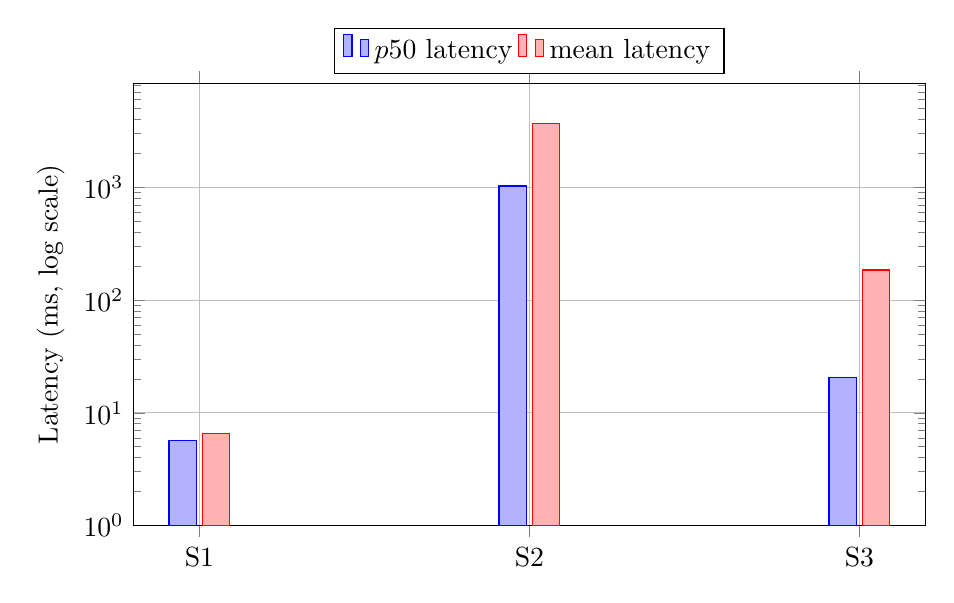
\begin{tikzpicture}
\begin{axis}[
    ybar,
    bar width=10pt,
    width=0.96\textwidth,
    height=7.2cm,
    symbolic x coords={S1,S2,S3},
    xtick=data,
    xticklabels={S1,S2,S3},
    ylabel={Latency (ms, log scale)},
    ymode=log,
    log basis y={10},
    ymin=1,
    grid=major,
    legend style={at={(0.5,1.02)}, anchor=south, legend columns=2}
]
\addplot coordinates {(S1,5.63) (S2,1028.92) (S3,20.71)};
\addplot coordinates {(S1,6.56) (S2,3695.97) (S3,184.70)};
\legend{$p50$ latency, mean latency}
\end{axis}
\end{tikzpicture}
\caption{Generative AI сценаруудын latency-ийн харьцуулалт}
\label{fig:genai_latency_compare}
\end{figure}

\begin{figure}[H]
\centering
\begin{tikzpicture}
\begin{axis}[
    ybar,
    bar width=16pt,
    width=0.82\textwidth,
    height=6.5cm,
    symbolic x coords={S1,S2,S3},
    xtick=data,
    xticklabels={S1,S2,S3},
    ylabel={CPU ачаалал (\%)},
    ymin=0,
    ymax=7,
    grid=major,
    nodes near coords,
    every node near coord/.append style={font=\scriptsize}
]
\addplot coordinates {(S1,5.92) (S2,0.37) (S3,1.74)};
\end{axis}
\end{tikzpicture}
\caption{Generative AI сценаруудын CPU ачааллын харьцуулалт}
\label{fig:genai_cpu_compare}
\end{figure}

S2 сценарт source тархалт нь \texttt{fallback\_activity\_pack\_fast}=1, \texttt{fallback\_local\_styled}=9 байв. Энэ нь гаднын зураг үүсгэх оролдлого амжилтгүй болох үед систем дотоод fallback руу автоматаар шилжиж байгааг бодит хэмжилтээр баталлаа.

Тайлбар: S2, S3 сценарт дундаж (mean) хугацаа $p95$-аас өндөр гарсан нь цөөн тооны маш урт хүсэлт (жишээ нь max=25964.18 ms) гарсантай холбоотой бөгөөд энэ нь гадаад сервисийн саатлын эрсдэлийг илэрхийлж байна.

\section{Хэрэглэгчийн интерфейс ба туршлагын ажиглалт (UI/UX)}

Хэрэгжилтийн туршид дараах хэрэглэгчийн туршлагын (UX) шийдлүүд эерэг нөлөө үзүүлсэн:

\begin{itemize}
    \item Ачааллын (loading) төлөв бүрт тодорхой заагч (indicator) ашигласан,
    \item Алдааны мессежийг хэрэглэгчид шууд ойлгомжтой байдлаар харуулсан,
    \item CRUD үйлдлийн дараа хэрэглэгчийн интерфейсийг (UI) автоматаар шинэчилж (refresh), өгөгдлийн зөрүүг бууруулсан,
    \item Сэтгэл хөдлөлийн төлөв (mood) болон дүрст тэмдэг (emoji) ашигласнаар тэмдэглэл оруулах оролцоо нэмэгдсэн.
\end{itemize}

\section{Эрсдэл ба хязгаарлалтын үнэлгээ}

Хэрэгжилтийн явцад илэрсэн гол хязгаарлалтууд:

\begin{enumerate}
    \item Сервер талд (backend) MONGO\_URI болон JWT\_SECRET-ийн анхдагч (fallback) утга ашиглаж байгаа нь үйлдвэрлэлийн орчинд (production environment) аюултай.
    \item OPENAI\_API\_KEY хамааралтай тул гадны үйлчилгээ тасалдах эрсдэлтэй.
    \item Мэдэгдлийн урсгал нь \texttt{/api/notes} өгөгдөл дээр клиент талд нэгтгэгдэж байгаа бөгөөд тусдаа мэдэгдлийн API болон алсын түлхэх мэдэгдлийн үйлчилгээ (FCM/APNs) үйлдвэрлэлийн түвшинд бүрэн нэгтгэгдээгүй.
    \item Токен шинэчлэх механизм (token refresh) хийгдээгүй тул урт хугацааны сешн удирдлага (session management) сайжруулах шаардлагатай.
\end{enumerate}

